%===================== CROSS-MEDIA LEARNING FOR IMAGE CLASSIFIERS =========================

\graphicspath{{img/vsa/}}

\newcommand{\BTSA}{B-T4SA}
\newcommand{\ourFtAlex}{Hybrid-T4SA}
\newcommand{\ourFtVGG}{VGG-T4SA}

\chapter{Weakly-supervised Cross-media Learning of Convolutional Neural Networks}
\label{ch:cross-media}

The most straightforward way to build a visual image classifier using \glspl{cnn} is to perform supervised learning.
While in previous work the cost of human interaction was spent on the manual engineering of features detectors and descriptors, this cost recently shifted to labeling of datasets in order to train deep models.
Even if the labeling task is simpler and more accessible, correctly labeling huge datasets is still a labor-intensive and expensive job, which is usually carried out by crowd-sourcing.
Current large-scale datasets, such as ImageNet, are in fact limited in their scalability due to the labeling cost on which their collectors incur.
Thus, the attention of recent research shifted to the exploitation of the huge amount of data coming from the web and social medias which became easily available in the last years~\cite{sun2017revisiting,mahajan2018exploring}.
The main objective is to reduce the amount of human interaction needed to train an image classifier and obtain good features by exploiting correlation that can emerge in large-scale datasets.
Despite having the advantage of being free and constantly growing, this source of data poses challenges in its usage, since it commonly presents noisy or incomplete information.
This usually limits the amount of supervision that can be extracted from this kind of data, but the possibility to scale the training procedures to huge amount of data often compensates this limitation.

In this chapter, we propose a novel weakly-supervised cross-media approach to train visual image classifiers in an autonomous way exploiting social media data.
We rely on textual data --- which usually accompanies images in social media posts --- to provide a noisy supervision in the training phase of a visual only classifier.
To exhibit the advantages of our approach, we employed it to tackle \emph{visual sentiment analysis} --- a problem in which the cost of data labeling is rather high --- using a large set of user-generated and unlabeled contents to train a \acrfull{dcnn}.
We demonstrated via experimental evaluation that models trained with our approach are able to extensively exploit the noisy information contained in uncontrolled social media data to build a visual sentiment polarity classifier with no human supervision that outperforms state-of-the-art approaches in visual sentiment analysis.
The data used in experiments --- collected from Twitter interrogating its Streaming API --- has been packed in a dataset and publicly released to foster new research on the field of visual sentiment analysis.

The chapter is structured as follows.
In \ref{sec:vsa:introduction}, the problem of visual sentiment analysis is presented, together with a discussion about the challenges it poses and an overview of the current state of the art.
\ref{sec:vsa:dataset} presents the methodology used to collect and preprocess the social media data used in our experiments.
In \ref{sec:vsa:method}, our weakly-supervised cross-media learning approach is described in detail, and \ref{sec:vsa:experiments} reports its experimental evaluation and comparison with state-of-the-art approaches to visual sentiment analysis.
\ref{sec:vsa:conclusion} summarizes the main findings and concludes the chapter.

The research presented in this chapter was published in~\cite{vadicamo2017cross}, and the provided resources --- e.g.\ datasets and trained models --- are available at \url{http://t4sa.it}.


%%% ABSTRACT
% Much progress has been made in the field of sentiment analysis in the past years. Researchers relied on textual data for this task, while only recently they have started investigating approaches to predict sentiments from multimedia content.
%With the increasing amount of data shared on social media, there is also a rapidly growing interest in approaches that work ``in the wild'', i.e. that are able to deal with uncontrolled conditions.
%In this work, we faced the challenge of training a visual sentiment classifier starting from a large set of user-generated and unlabeled contents.
%In particular, we collected more than 3 million tweets containing both text and images, and we leveraged on the sentiment polarity of the textual contents to train a visual sentiment classifier.
%To the best of our knowledge, this is the first time that a cross-media learning approach is proposed and tested in this context.
%We assessed the validity of our model by conducting comparative studies and evaluations on a benchmark for visual sentiment analysis.
%Our empirical study shows that --- although the text associated to each image is often noisy and weakly correlated with the image content --- it can be profitably exploited to train a deep Convolutional Neural Network that effectively predicts the sentiment polarity of previously unseen images.

\section{Visual Sentiment Analysis}
\label{sec:vsa:introduction}

Recent years experienced a rapid and increasing adoption of social media as information exchange and communication platforms.
On a daily basis, users generate and share a large quantity of multimedia content --- such as texts, images, and videos --- which conveys information about their opinions about a vast range of topics.
The availability of such a source of data attracted the scientific community as well as the industries to large-scale sentimental analyses of the public opinion.
Opinion mining and sentiment analysis~\cite{pang2008opinion} foster applications in multiple domains, such as market prediction~\cite{mishne2006predicting,asur2010predicting}, government intelligence~\cite{abbasi2007affect}, political elections~\cite{laver2003extracting,o2010tweets}, and crisis management~\cite{avvenuti2016impromptu,cresci2015linguistically}, to name a few.

Thanks to the multi-modality of modern social platforms, current trends show that visual media are increasingly chosen due to their immediate and effective communication, and less and less text is written by users.
Therefore, researchers shifted their attention from a pure textual-based sentiment analysis presented in seminal work to a multi-modal analysis which includes also visual information conveyed by images and videos~\cite{borth2013large,cao2016cross,jou2015visual,siersdorfer2010analyzing,you2015robust,you2016cross}.
In particular, we identify as \emph{visual sentiment analysis} the task of extracting subjective information --- such as emotions and opinions --- solely from visual data.
Understanding the content of a piece of visual information is an objective task, and much progress has been made in the computer vision research community to accurately describe visual contents, i.e.\ reducing the semantic gap between image representations and content~\cite{li2016socializing}.
However, describing the emotions arisen in human observers is challenging due to the highly subjectivity involved.
This discrepancy between the affective content of an image and its description --- known as the \emph{affective gap}~\cite{siersdorfer2010analyzing} --- poses considerable challenges to visual sentiment analysis.
This difficulty is also reflected on the generation of labeled sets for training sentiment classifiers;
several emotional judgements by multiple annotators are usually required to obtain a high-quality sentiment groundtruth for a single image, thus increasing the cost of dataset creation.

While in general sentiment analyses can tailor a large range of emotions, the commonly adopted form of sentiment analysis is the determination of the sentiment polarity of a piece of information, i.e.\ an indicator of the emotional positiveness or negativeness conveyed.
As the vast majority of attempts in the literature, our work is framed in this formulation;
thus, our goal is to predict the sentiment polarity of a given image. % TODO better justify
% \subsection{Related Work} \label{sub:vsa:rel-work}
In the next paragraphs, we will provide the reader with an overview of existing work on sentiment analysis with emphasis on the ones based on visual data.

\paragraph{Text-based Sentiment Analysis}
%For what concerns the detection of sentiment polarity in texts extracted from Twitter, first works considered simple linguistic features, such as word unigrams, word bigrams and parts-of-speech, using machine learning algorithms like Naive Bayes, Maximum Entropy and \acrfullpl{svm}.
Seminal works on sentiment polarity estimation from textual data~\cite{go2009twitter,bermingham2010classifying} employed classic \gls{ml} algorithms which relied on simple linguistic features --- such as word n-grams and part-of-speech.
%In the last few years, deep neural networks contributed to considerable performance improvements with respect to other popular learning algorithms, such as \glspl{svm}.
Subsequently, deep learning approaches positively contributed with more accurate models for text analysis and natural language processing, which in turn gave a huge contribution in textual sentiment analysis.
%In particular, \acrfullpl{lstm}, which we also employ in this work, and \acrfullpl{cnn} were tested on several shared tasks, such as the Semeval Sentiment analysis in Twitter \cite{nakov2016semeval}, which is considered by the Natural Language Processing community the most important benchmark for this task.
%The results obtained by the submitted systems, such as the ones by \citet{deriu2016swisscheese} and \citet{rouvier2016sensei}, have shown that the combination of these learning techniques with the adoption of word embeddings, a compact real-value vector word representation which takes into account word similarity \cite{mikolov2013distributed,pennington2014glove}, is able to set the state-of-the-art with minimal feature engineering, which makes such architectures more robust and flexible than previous ones.
The Semeval Sentiment analysis in Twitter \cite{nakov2016semeval} challenge is a testimony of this influence: an increasing number of submitted solutions~\cite{deriu2016swisscheese,rouvier2016sensei} combined the power of deep models --- such as \acrfullpl{lstm} and \acrfullpl{cnn} --- and word embeddings~\cite{mikolov2013distributed,pennington2014glove} to set the state of the art with minimal or no feature engineering.

% ---

\paragraph{Visual Sentiment Analisys}
While there is a large literature on extracting emotional information from textual content, research on image-based sentiment analysis is still in its early stages.
First approaches to infer affects from images were based on supervised or semi-supervised frameworks that map low-level features of images into human emotions \cite{machajdik2010affective,siersdorfer2010analyzing,jia2012can}.
 \citet{siersdorfer2010analyzing} firstly applied and evaluated automatic classification of sentiment using a large-scale collection of photos crawled from Flickr using the SentiWordNet \cite{esuli2007sentiwordnet} dictionary as query terms. % NOELAB
They used pixel-level color histogram and SIFT-based Bag-of-Word representations as visual features and trained a \gls{svm} to predict the sentiment of images. % NOELAB
To overcome the \emph{affective gap} between low-level features and emotional content of an image, \citet{borth2013large}, \citet{yuan2013sentribute} and \citet{jou2015visual} employed visual entities or attributes to extract mid-level visual representations.
The main contribution of~\cite{borth2013large} and~\cite{jou2015visual} was building a large scale visual sentiment ontology, called VSO and Multilingual VSO, respectively, which consist of thousands of semantic objects (Adjective Noun Pairs -- ANP) strongly linked to emotions.
Using their ontologies, they also proposed  a bank of detectors, namely \emph{SentiBank} and \emph{MVSO}, that can automatically extract these mid-level representations.
%For example, Sentibank detects the responses of 1200 ANP concepts in an image, which means that it represents each image by a 1200-dimensional vectors of responses.
For the sentiment prediction task, a classifier is learned on the top of these mid-level representations that are used as image features.
This means that the ANP's textual sentiments are not explicitly used for the sentiment prediction.
Just recently, \citet{li2018image} investigated the fusion of the sentiment prediction obtained using \emph{ANP responses as image features} with the sentiment prediction obtained using the \emph{ANP's textual sentiment values}.
\citet{chen2014deepsentibank} proposed an improved version of SentiBank, called \emph{DeepSentiBank} which exploit \acrfullpl{dcnn} to build a visual sentiment concept classification model.
The approaches used in \cite{jou2015visual,li2018image} relied on deep learning algorithms, which recently have significantly changed the research landscape in a broad set of domains, such as visual object recognition and image classification. %, and text classification.
%In the last years, deep learning approaches \cite{lecun2015deep} have dramatically improved the state-of-the-art in many domains, such as visual object recognition, image classification, speech recognitions and text classification.
Following the success of deep learning, many other approaches based on deep neural networks have been proposed for visual sentiment prediction and image emotion classification \cite{campos2017pixels,chen2014deepsentibank,islam2016visual,rao2016learning,you2015robust,xu2014visual}.
Most of these have in common the use of \glspl{cnn} trained or fine-tuned on sentiment-related and labeled data.
In \cite{campos2017pixels,chen2014deepsentibank,islam2016visual,jou2015visual}, %,xu2014visual %sun2016discovering %VGGNet \cite{simonyan2014very}
state-of-the-art \gls{cnn} architectures --- such as AlexNet~\cite{krizhevsky2012imagenet}, PlaceCNN~\cite{zhou2014learning}, and GoogleNet \cite{szegedy2015going} --- were exploited.
\citet{you2015robust} proposed a custom \gls{cnn} architecture specifically designed for visual sentiment prediction.
Since their network was trained on weakly labeled images, they also proposed an approach, called PCNN, to reduce the impact of noisy training images. %instances by progressively select a subset of the training images.
\citet{sun2016discovering} boosted the performance of CNNs by selecting affective local regions of the images which are likely containing objects and carrying massive emotions. % NOELAB

\paragraph{Multi-modal Sentiment Analysis}
There are also several publications on analyzing sentiments using multi-modalities, such as text and image.
For example, \citet{cao2016cross} proposed a late fusion to combine the predictions obtained from text and image, while \citet{you2016cross} proposed a cross-modality consistent regression (CCR) scheme for joint textual and visual analysis.
Recently, multi-modal learning approaches have been proposed for joint textual and visual understanding.
\citet{baecchi2016multimodal} proposed a multi-modal feature learning schema based on CBOW and denoising autoencoders to perform sentiment analysis.
In \cite{mao2014deep}, the authors proposed a deep end-to-end architecture where each modality is encoded is an appropriate sub-network (an \gls{rnn} for text and a \gls{cnn} for images) and then fused in a multi-modal layer.
Similarly, \citet{ma2015multimodal} encodes both modalities with convolutional networks.

Differently from all the approaches previously presented, in our work we are interested in (i) understanding human sentiments by exploiting a large-scale dataset of unlabeled images collected from social-media, (ii) training sentiment classifiers without any prior knowledge of the collected data.
Although textual information accompanying social media images is often incomplete and noisy, it can be effectively exploited to enable unsupervised sentiment analysis.
A first step in this direction was taken in \cite{wang2015unsupervised} where an Unsupervised SEntiment Analysis (USEA) for social-media images based on nonnegative matrix factorization was proposed.
Our work differs from that of \citet{wang2015unsupervised} in the way of exploiting the textual information and in the final classifier.
In fact, we train a deep neural network that can be used to predict the sentiment of any new image \emph{without} using any textual information for those images, while USEA infers sentiments for images by \emph{jointly} considering visual and textual information.
%Moreover, Wang \etal  did not test their approach on hand-labeled images or benchmarks for visual sentiment analysis for further comparisons.

%-------------------------------------------------------------------------

In this paper, we focus on discovering the sentiment polarity (\emph{positive}, \emph{negative} or \emph{neutral}) of a given image.
We follow the current trend of facing sentiment ``in the wild", that is, in all sort of varying conditions of the everyday world that we share with others (as opposed to testing situation in laboratories).
For this scope, social networks, such as Twitter and Facebook, are particularly suitable as sources of data for our analysis, thanks to the huge variation of contents shared by their users.

The vast majority of the existing visual sentiment classifiers have been trained on sentiment-related images, typically annotated using crowd-sourcing. %State-of-the-art approaches are based on deep learning model which need huge volume of training labeled data that is difficult to collect. In this work, we exploit deep learning models to build our visual sentiment classifiers.
As other state-of-the-art approaches, we exploit deep learning models to build our visual sentiment classifiers.
However, differently from previous supervised approaches, we propose an end-to-end pipeline to train the visual classifier starting from a large-scale dataset of unlabeled tweets (text and images). %we collected from Twitter.
First, we use a tandem Long Short Term Memory Recurrent Neural Network-Support Vector Machine (LSTM-SVM) architecture to classify the sentiment polarity of the texts.
Then, we exploit the images of the tweets, labeled according to the sentiment polarity of the associated text, to fine-tune a deep Convolutional Neural Network (CNN) architecture, by leveraging on transfer learning.
Although the text of the tweets is often noisy or misleading with respect to the image content (\eg irrelevant comments), we show that our cross-media approach can be profitably used for learning visual sentiment classifiers in the wild.
In fact, our results on a manually annotated benchmark for visual sentiment analysis %\cite{you2015robust}
show that the prediction accuracy of our trained CNN models is better than, or in the worst cases, in line with, state-of-the-art classifiers trained on sentiment-related data sets. %~\cite{borth2013large,Campos2016,islam2016visual,siersdorfer2010analyzing,you2015robust,yuan2013sentribute}.

The main contributions of our work can be summarized as follows:
\begin{itemize}
  \item %We address the challenges of visual sentiment analysis in the wild,
  We present an empirical study to analyze visual sentiments in the wild,
  %using
  starting from a large-scale dataset of \emph{unlabeled} user-generated content.
  To the best of our knowledge, this is the first work that proposes %an ``unsupervised" and data-driven approch
  a cross-media approach to learn a classifier for predicting the sentiment polarity of a given image.
  In particular, we show that we are able to train visual sentiment classifiers that are comparable to, or better than, state-of-the-art classifiers trained on sentiment-related labeled images.
  \item Overall, we collected and analysed more that 3 million tweets in order to construct the \emph{\acrfull{t4sa}} dataset.
  \gls{t4sa} is composed of about 1 million high-confidence tweets for which we provide the textual sentiment classification, and the corresponding 1.4M images.
  We make all the collected tweets as well as the \gls{t4sa} dataset publicly available to encourage further research \footnote{http://www.t4sa.it}.
  %We construct \emph{\NomeTSA} (\TSA) dataset, composed of more than X million tweets for which we provide the textual sentiment classification and the corresponding XXM images. We make  the dataset publicly available to encourage further research\footnote{This is an Anonymised Link}.
%   We construct {\NomeInitialDatset} (\NID) dataset, composed of {\color{blue}XXX} tweets for which we provide the textual sentiment classification and the corresponding {\color{blue}XXX (qui serve il numero di immagini prima del filtraggio di Felice)} images. We make  the dataset publicly available to encourage further research\footnote{This is an Anonymised Link}.}
  \item We publicly release our trained visual sentiment classifiers, namely  \emph{\ourFtAlex}\, and \emph{\ourFtVGG}, %\footnote{http://www.t4sa.it},
  and we conduct comparative studies and evaluations on benchmarks for visual sentiment analysis.
\end{itemize}

%-------------------------------------------------------------------------

\section{Data Collection}
\label{sec:vsa:dataset}
Both the textual and the multimedia data used in this work have been collected from Twitter, by means of a streaming crawler. The data collection process took place from July to December 2016, lasting around 6 months in total. During this time span we exploited Twitter's Sample API\footnote{https://dev.twitter.com/streaming/reference/get/statuses/sample} to access a random 1\% sample of the stream of all globally produced tweets. All the tweets collected in this way have undergone a filtering step where we have applied a set of simple rules in order to retain only data that could be useful for our sentiment analysis task. Specifically, we discarded:
\begin{enumerate}
\item\label{filter:retweets} retweets;
\item\label{filter:images} tweets not containing any static image (i.e., we also discarded tweets containing only videos and/or animated GIFs);
\item\label{filter:english} tweets not written in the English language;
\item\label{filter:length} tweets whose text was less than 5 words long.
\end{enumerate}
Rules~\ref{filter:retweets} and~\ref{filter:images} help increasing the quality of collected multimedia data.
In detail, enforcing Rule~\ref{filter:retweets} avoids collecting large numbers of duplicated images, while Rule~\ref{filter:images} ensures that each collected tweet have at least a static image for the visual sentiment classification task. Rules~\ref{filter:english} and~\ref{filter:length} are instead aimed at guaranteeing that we have enough textual data for the textual sentiment classification task.

The above set of rules filtered as much as 98.7\% of all the tweets collected from the Twitter stream. Anyway, the huge volume of tweets produced globally still allowed to collect a stream of more than 43 useful (i.e., not filtered out) tweets per minute, on average. At the end of the data collection process, the total number of tweets in our dataset
is $\sim$ 3.4M, corresponding to $\sim$ 4M images. Then, we classified the sentiment polarity of the \emph{texts} (as described in Section \ref{sec:text}) and we selected the tweets having the most confident textual sentiment predictions to build our \emph{\acrfull{t4sa}} dataset. \gls{t4sa} contains %$2,140,711$
%$\sim$ XXM tweets, corresponding to $\sim$  XXM images.
little less than a million tweets, corresponding to $\sim$ 1.5M images.
We publicly release {all the collected tweets} and the \gls{t4sa} dataset.% as incentive for future research and applications.
%{\color{blue} TODO: cambiare il testo a seconda che si diano tutti i tweets o solo quelli annotati con high confidence}


%-------------------------------------------------------------------------
\section{From Textual to Visual Sentiment Analysis}
\label{sec:vsa:method}
%\section{Text Analysis}\label{sec:text}
%qui tagliati settegli tecnici o
The text extracted from the collected tweets has been classified according to the sentiment polarity using an adapted version for the English language of the ItaliaNLP Sentiment Polarity Classifier~\cite{cimino2016tandem}.
This system was successfully employed in the SENTIment POLarity Classification task~\cite{barbieri2016overview}, which was organized within Evalita 2016, the 5th evaluation campaign of Natural Language Processing and Speech tools for Italian.
This classifier is based on a tandem LSTM-SVM architecture.
SVM classification algorithms use ``sparse" and ``discrete" features in document classification tasks, making really hard the detection of relationships in sentences, which is often the key factor in detecting the overall sentiment polarity in documents~\cite{tang2015document}.
On the contrary, LSTM networks are a specialization of Recurrent Neural Networks (RNN) which are able to capture long-term dependencies in a sentence. This type of neural network was recently tested on Sentiment Analysis and proved to outperform previous systems \cite{nakov2016semeval}.
%, showing a 3-4 points improvements with respect to other commonly used learning algorithms.
In this work, the tandem system uses LSTM to  learn  the  feature  space and to  capture temporal dependencies, while the SVMs are used for classification.
SVMs combine the document embedding produced  by  the  LSTM  in conjunction with  a  wide  set of general-purpose features qualifying the lexical  and grammatical  structure  of  the text.

We  employed  a  bidirectional  LSTM (bi-LSTM) architecture since these kind of architecture allows to capture long-range dependencies from both directions
of a document by constructing bidirectional links in the network \cite{schuster1997bidirectional}.

In the training phase, the bi-LSTM network is trained considering the training documents and the corresponding gold labels. Once the statistical model of the bi-LSTM neural network is computed, for each document of the training set, a document vector (document embedding) is computed exploiting the weights that can be obtained from the penultimate network layer (the layer before the
SoftMax classifier) by giving in input the considered document to the LSTM network. The document embeddings are used as features during the training phase of the SVM classifier in conjunction  with  a  set  of  widely  used  document  classification features. Once the training phase of the SVM classifier is completed the tandem architecture is considered trained. The  same stages are involved in the classification phase: for each document an embedding vector is obtained exploiting the  previously trained LSTM network. Finally the embedding is used jointly with other document classification features (see Section \ref{exp:visual} for further details) by the SVM classifier which outputs the predicted class.

In order to evaluate the performance of our Sentiment Classifier, we performed a 10-fold cross validation over 6,293 tweets belonging to the dataset distributed for the SemEval-2013 Task on Sentiment Analysis in Twitter. We used a subset (approximately the 60\%) of the original dataset since at the time we downloaded the tweets through the scripts provided by the task organizers, just a subset of all the dataset was still available in Twitter. Our classifier reported an average F1-score of 66.15. This result is particularly good considering that the winner of the competition, the NRC-Canada team \cite{mohammad2013nrc}, achieved a F1-score of 69.02 using \emph{all} the available training data.
%%

Our Sentiment Classifier was used to analyze the text of a large set of user-generated multimedia contents (containing both text and images). We selected data with the most confident textual sentiment predictions and we used these predictions to automatically assign sentiment labels to the corresponding images. The aim was to automatically build a training set for learning a \emph{visual} classifier able to discover the sentiment polarity of a given image.
%The text analysis have been used to build our dataset \gls{t4sa} by selecting tweets with the most confident textual sentiment predictions. The aim was  to automatically build a training set for learning a \emph{visual} classifier able to discover the sentiment polarity of a given image.
%%-------------------------------------------------------------------------
%\section{Image Analysis} % ISTI
%In our framework, we are interested in discovering the sentiment polarity of a given image.
We modeled this task as a three-way image classification problem in which each image
can be classified as either \emph{positive}, \emph{neutral}, or \emph{negative}. We exploited
deep Convolutional Neural Networks (CNNs) as trainable classifiers due to their effectiveness
in numerous vision tasks \cite{amato2017deep,amato2016visualabbasi2007affect,krizhevsky2012imagenet,sharif2014cnn,simonyan2014very}. %girshick2014rich %%taglio
Deep CNNs allow a machine to automatically learn representations of data with multiple levels of abstraction that can be used for detection or classification tasks.
% dcnn as learnable classifier
A deep CNN is a feed-forward neural network composed of a possibly large number of convolutional layers with learnable filter banks
that can be seen as a trainable stack of feature extractors. Each layer of a deep network extracts useful knowledge
from its input to generate a feature with a higher level of abstraction, and all the layers are jointly optimized
using backpropagation in order to predict difficult high level concepts directly from pixels.
Convolutions are particularly suitable for visual data, since they are able to model the spatial correlation
of neighboring pixels better than normal fully connected layers. For a classification problem,
the final outputs of the CNN are the confidences for each class the network has been trained on.
% transfer learning and finetuning of a dcnn
% TODO spiegare transfer learning un minimo

To build our visual classifier, we leveraged on transfer learning. We used  a balanced subset of our dataset \gls{t4sa}
to {fine-tune} known and successful deep CNNs architectures pretrained on generic datasets of images. Doing so, we are able to exploit additional knowledge already stored in the trained network while training for sentiment prediction. In particular, we used \emph{HybridNet}~\cite{zhou2014learning} and \emph{VGG-19}~\cite{simonyan2014very} models.
% %_____________tagliati baseline technical details_____________
% The architecture of \emph{HybridNet} %is the same of the \emph{BVLC Reference CaffeNet}~\cite{jia2014caffe}, which
% mimics the original AlexNet \cite{krizhevsky2012imagenet} with minor variations as described in~\cite{zhou2014learning}. %\cite{jia2014caffe}.
% It has $8$ weight layers: $5$ convolutional and $3$ fully-connected. The model {was} trained on $1,183$ categories ($205$ scene categories from Places205~\cite{zhou2014learning} and $978$ object categories from the train data of ImageNet~\cite{russakovsky2015imagenet}) with about $3.6$ million images.
% The \emph{VGG-19} is an improved version of the model used by the VGG team of the University of Oxford in the ILSVRC-2014 competition, as described in \cite{simonyan2014very}. The model {was} trained on $1,000$ categories of ImageNet~\cite{russakovsky2015imagenet} with about $1.5$ million images. It contains $19$ weight layers ($16$ convolutional + $3$ fully-connected).
% %________________________________________________________
% Both the pre-trained models can be downloaded from the \emph{Caffe Mode Zoo} \footnote{\url{http://caffe.berkeleyvision.org/model_zoo.html}}.
In Section~\ref{exp:visual}, we describe the fine-tuning process used for building our visual sentiment classifiers.

%-------------------------------------------------------------------------
\section{Experimental Evaluation}
\label{sec:vsa:experiments}
\subsection{Dataset Preparation}
% \begin{table*}[t]
% \renewcommand{\arraystretch}{1.2}
% \begin{center}
% \small{\begin{tabular}{
% |>{\raggedright\arraybackslash}p{0.1\textwidth}
% |>{\raggedleft\arraybackslash}p{0.09\textwidth}
% >{\raggedleft\arraybackslash}p{0.09\textwidth}
% |>{\raggedleft\arraybackslash}p{0.165\textwidth}
% |>{\raggedleft\arraybackslash}p{0.08\textwidth}|
% }
% \hline
% \multirow{2}{*}{\textbf{Sentiment}} & \multicolumn{2}{c|}{\multirow{2}{*}{\textbf{\TSA}}} & {\textbf{\TSA} \footnotesize{w/o corrupted and near-duplicate images}} & \multirow{2}{*}{\centering\textbf{\BTSA}}\\
% %\cline{2-3}
% & {\footnotesize\emph{(tweets)}} & {\footnotesize\emph{(images)}}& {\footnotesize\emph{(images)}}& {\footnotesize\emph{(images)}}\\
% \hline\hline
% Positive & 572,749 & 738,415 & $556,335$ & $156,862$ \\
% Neutral & 1,388,912 & 1,619,075 & $1,043,477$ & $156,862$ \\
% Negative & 179,050 & 214,462  & $156,862$ & $156,862$  \\ \hline
% Sum & 2,140,711 & 2,571,952 & $1,756,674$	& $470,586$ \\
% \hline
% \end{tabular}}
% \end{center}
% \caption{Our \NomeTSA\, (\TSA) dataset ans its subsets used for learning the visual classifiers. Please note that each tweet (text + associated images) is labeled according to sentiment polarity of the text predicted using our tandem Long Short Term Memory Recurrent Neural Network (LSTM) - Support Vector Machines (SVM) architecture.} \label{tab:TSA}
% \end{table*}
All the $\sim$3.4M tweets collected as reported in Section \ref{sec:data} were analyzed by the textual sentiment polarity classifier described in Section \ref{sec:text}. In order to produce a reliable dataset for learning a visual sentiment classifier, we selected only the tweets classified with a confidence $\geqslant 0.85$\footnote{Using this threshold, the classifier achieves state of the art accuracy of 0.71 in terms of F-score.}. The resulting dataset contains $371,341$ Positive, $629,566$ Neutral, and $31,327$ Negative tweets. As expected, the dataset proved to be very imbalanced, a frequent and known issue in social media sentiment data \cite{li2011semi}. In order to increase the number of Negative tweets we selected a lower filtering threshold for this class, obtaining $179,050$ examples.
Notably, in our experiments conducted on \gls{t4sa}, the difference in precision on the classification of positive, neutral, and negative never exceeds $1\%$ and thus, the lower threshold used for selecting negative examples did not impact the quality of the learning.
Starting from this dataset, we selected a balanced subset of images to train visual sentiment classifiers.
To do so, we performed the following steps:
\begin{itemize}
\item %We selected from the collected data the tweets having the most confident textual sentiment predictions, for a total of $x$ tweets corresponding to $x$ images.
We labeled each image of \gls{t4sa} on the basis of the corresponding textual sentiment classification.
\item We removed corrupted and near-duplicate images resulting in %$1,756,674$
$\sim$ 974K unique images.
\item We selected a \emph{balanced} subset composed by $156,862$ images for each class, resulting in $470,586$ images. We call this subset {\BTSA}.
\item We split {\BTSA} in training, validation and test subsets, corresponding approximately to 80\%, 10\%, and 10\% of the images. %composed respectively by $368, 586$, $51,000$ and $51,000$ images.
\end{itemize}

\begin{table}
\centering
\newcolumntype{R}{>{\raggedleft\arraybackslash}X}
\begin{tabularx}{\linewidth}{lRRRR}
\toprule
                    & \multicolumn{2}{c}{\textsc{T4SA}} & \textsc{T4SA} {\footnotesize (no dup.)} & \textsc{B-T4SA} \\
                      \cmidrule(lr){2-3}                  \cmidrule(lr){4-4}      \cmidrule(lr){5-5}
\textsc{Sentiment}  & \textsc{tweets} & \textsc{images} & \textsc{images}       & \textsc{images} \\
\midrule
Positive            &  371,341        &   501,037       & 372,904               & 156,862 \\
Neutral             &  629,566        &   757,895       & 444,287               & 156,862 \\
Negative            &  179,050        &   214,462       & 156,862               & 156,862 \\
\midrule
Sum                 &  904,395        & 1,473,394       & 974,053               & 470,586 \\
\bottomrule
\end{tabularx}
\caption{Our \acrfull{t4sa} dataset and its subsets used for learning our visual classifiers. Each tweet (text and associated images) is labeled according to the sentiment polarity of the text, predicted by our tandem LSTM-SVM architecture.}
\label{tab:TSA}
\end{table}

Details on \gls{t4sa} and its subsets are summarized in Table \ref{tab:TSA}.
Notice that the size of the balanced subset (i.e., {\BTSA}) was highly influenced by the low number of tweets classified as negative. Moreover, these negatives contain many artificial images (\eg screenshots and memes), which made our analysis more challenging.   %or noisy label (due to the lower threshold used for selecting the negative samples). This made our analysis more challenging.
In fact, we encountered difficulties in automatically collecting negative tweets that also contain natural images by using only a random sample of all globally produced tweets. However, in order to avoid possible biases in our analyses, we deliberately avoided to use any keyword during the data collection process.


%Notice that the size of {\BTSA}, and so of the training set, was highly influenced by the low number of tweets classified as negative, and that many of these contain artificial images (\eg screenshots and memes) or  noisy label due to the lower threshold used for selecting the  negative samples.
%
%In fact, We observed a lower propensity of Twitters users to share negative post with natural images, which made our analysis more challenging.


%-----------------------------------------------------------------------------
\subsection{Experimental Settings}
\label{exp:visual} % ISTI (Fabio)
\paragraph{Text Analysis Settings}
As described in Section \ref{sec:text}, we employed a bidirectional LSTM to learn a document embedding into a feature space.  We  applied  a  dropout  factor of 0.45 to both input  gates and to the recurrent connections in order to prevent  overfitting,  a  typical  issue  in  neural networks ~\cite{gal2016theoretically}. For  what  concerns  the  optimization process, categorical cross-entropy is used as a loss function and optimization is performed by the \emph{rmsprop} optimizer \cite{tieleman2012lecture}. We used the Keras \cite{libkeras} deep learning framework to develop the LSTM network.

Each input word to the LSTM is represented by a low dimensional, continuous and real-valued vector, also known as word embedding~\cite{MikolovSCCD13}, and all the word vectors are stacked in a word embedding matrix. For this work, we used GloVe~\cite{pennington2014glove} pre-trained vectors since these are computed considering the word context information. GloVe website~\footnotetext{http://nlp.stanford.edu/projects/glove/} provides freely available pre-trained vectors computed from a 2B English tweets corpus.

The document embedding produced by the LSTM is used in conjunction with other document  features by the SVM classifier.
The other document features %used by the SVM
focused on a wide set of features ranging across different levels of linguistic description. The features are organised into three main  categories: raw  and  lexical  text  features, morpho-syntactic features and lexicon features. With the exception  of the lexicon features, these features were already tested and described in \cite{cimino2016tandem}. To extract the lexicon features we exploited three freely available resources: The Bing Liu Lexicon~\cite{hu2004mining}, which includes approximately 6,000 English words, the Multi-Perspective Question Answering Subjectivity Lexicon~\cite{wilson2005recognizing}, which consists of approximately 8,200 English words, and the SentiWordNet 3.0 Lexicon~\cite{baccianella2010sentiwordnet} that consists of more than 117,000 words. For each word in these lexicons the associated polarity is provided. In addition, we manually developed a lexicon of positive and negative emoticons, which are usually a strong indicator of tweet polarity. By exploiting the described resources, the following features were extracted: positive/negative emoticon distribution, sentiment polarity n-grams, sentiment polarity modifiers, the distribution of sentiment polarity, the most frequent sentiment polarity and changes of polarity in tweet sections. The last lexicon feature is calculated using the word embedding produced by Glove and it is obtained by computing separately the average of the word embeddings of the nouns, adjectives, and verbs of the tweet.
\paragraph{Image Analysis Settings}
We used {\BTSA} training subset to fine-tune two different pretrained networks, namely:
AlexNet pretrained on ILSVRC2012 \cite{russakovsky2015imagenet} + Places205 \cite{zhou2014learning} (also called HybridNet \cite{zhou2014learning}) and VGG-19 \cite{simonyan2014very} pretrained
on ILSVRC2012 \footnote{Both the pre-trained models can be downloaded from the \emph{Caffe Mode Zoo} (\url{http://caffe.berkeleyvision.org/model_zoo.html})}.
We replaced the last fully connected layer \emph{fc8} %originally having 1000 outputs
with a new one having 3 outputs, and we experimented two % or N? to decide
different fine-tuning strategies we named \emph{FT-F} and \emph{FT-A}. In \emph{FT-A} we fine-tune all
the trainable layers, while in \emph{FT-F} the parameters of convolutional layers are fixed and
only the last fully connected layers \emph{fc6-8} are trained.
%In \emph{FT-C} we keep the first three convolutional layer fixed (or the first three groups of convolutions for the VGG-19) and we finetune layers from \emph{conv4} to the end of the networks.

We trained both networks with both the fine-tune strategies using Caffe \cite{jia2014caffe}
for $15$ epochs using SGD with momentum $\mu = 0.9$, a learning rate of $0.001$ divided by $10$ every $5$ epochs,
and L2 regularization with a weight decay of $10^{-5}$. For HybridNet %AlexNet
we used a batch size of $128$,
while for VGG-19 we used a batch size of $32$ and batch accumulation of $2$ to lower the
GPU memory footprint.

We assessed the performance of our models using our \BTSA\, test set and the so-called Twitter Testing Dataset presented in \cite{you2015robust}. The latter contains a total of $1,269$ images having a positive or negative sentiment that have been manually labeled by five Amazon Mechanical Turk (AMT) workers. The images are partitioned into three subsets, namely ``Five agree", ``At least four agree", and ``At least three agree", on the basis of the labeling results from the five AMT workers. The details of this dataset are reported in Table~\ref{TwitterTestingDataset}. %The Twitter Testing Dataset
Twitter Testing Dataset was also used in \cite{campos2017pixels,islam2016visual,li2018image,you2015robust}, allowing for a through comparison of our systems with the state-of-the-art. %sun2016discovering

\begin{table}
\centering
\newcolumntype{R}{>{\raggedleft\arraybackslash}X}
\begin{tabularx}{\linewidth}{lRRR}
\toprule
                   & \multicolumn{3}{c}{\textsc{Twitter Testing Dataset}} \\
                     \cmidrule(lr){2-4}
\textsc{Sentiment} & \textsc{5 agree} & \textsc{$\geq 4$ agree} & \textsc{$\geq 3$ agree} \\
\midrule
Positive           & 581              & 689                              & 769   \\
Negative           & 301              & 427                              & 500   \\
\midrule
Total              & 882              & 1,116                            & 1,269 \\
\bottomrule
\end{tabularx}
\caption{Twitter Testing Dataset \cite{you2015robust}.} \label{TwitterTestingDataset}
\end{table}

\subsection{Results}
In Table \ref{tab:Twitter882}, we reported the accuracy % and ...? other stuff we have to decide!
obtained by the fine-tuned models in our \BTSA\, test set and in all the subsets provided by the Twitter Testing Dataset.
\begin{table}
    \centering
    \newcolumntype{R}{>{\raggedleft\arraybackslash}X}
    \begin{tabularx}{\linewidth}{lRRRR}
    \toprule
                                & \multicolumn{3}{c}{\textsc{Twitter Testing Dataset}} & \multicolumn{1}{c}{\textsc{B-T4SA TEST}} \\
                                & \multicolumn{3}{c}{{\small (pos, neg)}}              & \multicolumn{1}{c}{{\small (pos, neu, neg)}} \\
                                  \cmidrule(lr){2-4}                                     \cmidrule(lr){5-5}
    \textsc{Model}              & \textsc{5 agree} & \textsc{$\geq 4$ agree} & \textsc{$\geq 3$ agree} & \\
    \midrule
    Random Classifier           & 0.500 & 0.500 & 0.500 & 0.333 \\
    CNN~\cite{you2015robust}   & 0.722 & 0.686 & 0.667 & -     \\
    PCNN~\cite{you2015robust}  & 0.747 & 0.714 & 0.687 & -     \\
    \ourFtAlex\, FT-F           & 0.766 & 0.748 & 0.723 & 0.499 \\
    \ourFtAlex\, FT-A           & 0.741 & 0.709 & 0.686 & 0.491 \\
    \ourFtVGG\, FT-F            & 0.768 & 0.737 & 0.715 & 0.506 \\
    \ourFtVGG\, FT-A            & \textbf{0.785} & \textbf{0.755} & \textbf{0.725} & \textbf{0.513} \\
    \bottomrule
    \end{tabularx}
	\caption{Prediction accuracy on the different test sets.} \label{tab:Twitter882}
\end{table}
As baseline references, we report the results obtained by a random classifier and by the CNN and PCNN models \cite{you2015robust}.
The results show that the models trained with our cross-media approach effectively classify the images of Twitter Testing Dataset which were manually annotated. In particular, our best model ({\ourFtVGG} FT-A) correctly classifies $78.5\%$ of the \emph{five agree} testing images, outperforming similar models trained on high-quality sentiment-related hand-labeled data~\cite{you2015robust}.
Since the Twitter Testing Dataset only provides binary labels (positive/negative) as groundtruth, we obtained a binary classification from our three-way model taking the maximum confidence between the positive and the negative confidences.
We also performed experiments using two-way fine-tuned nets trained only on positives and negatives images provided by our training set, but we observed that there is no significant difference in performance with respect to predictions derived from three-way models.
% Moreover, despite the presence of noisy labels especially for negative training images, our best model obtain similar F1 scores for both the positive (0.83) and negative (0.72) classes, meaning that is not too much biased towards a particular class.

Notice that the range of the accuracy values obtained on our \BTSA\, is lower because those experiments concern a three-way classification. Moreover, the groundtruth for the evaluation is not hand-labeled since it is derived from the analysis of the textual information collected ``in the wild", thus it contains noisy labels that inevitably lower the accuracy upper bound. %(see Figure \ref{fig:confusion-images}).
Figure \ref{fig:confusion-images} reports the most confident classifications on this test set. From a qualitative point of view, in several cases the sentiment polarity of the images is better represented by the prediction of our model than the sentiment polarity inferred from the text associated to the images. Since the textual sentiment analysis was used to label both testing and training images, this, on one hand, explains the relatively lower accuracy obtained by our models on the {\BTSA} test set and, on the other hand, confirms that we used sufficiently large set of training data to allow the deep neural network to handle noisy labels.
Moreover, we observed that the use of the \emph{neutral} class is particularly suitable for analyzing web images, which often depict simple objects or commercial products. For this reason we used a three-way model, unlike other state-of-the-art approaches which use a binary classification model~\cite{campos2017pixels,islam2016visual,you2015robust}.

% Many papers on visual sentiment analysis also report the 5-fold cross-validation accuracy on the Twitter Testing Dataset \cite{Campos2016,islam2016visual,li2018image,you2015robust}, in which the prediction of each fold is computed with a model fine-tuned on the other four folds. This measure tends to highlight how well a pretrained model adapts to a specific task or dataset. While we think that this measure is inappropriate for our cross-media approach, we also report it in Table \ref{tab:Twitter882_5fold} for comparison with other state-of-the-art methods.
% As evidenced by the results, the 5-fold accuracy of models trained on generic (not sentiment-related) datasets, like AlexNet and VGG-19, are comparable to the ones of the same models that have been previously finetuned on a sentiment-related dataset.

\begin{figure}
\centering
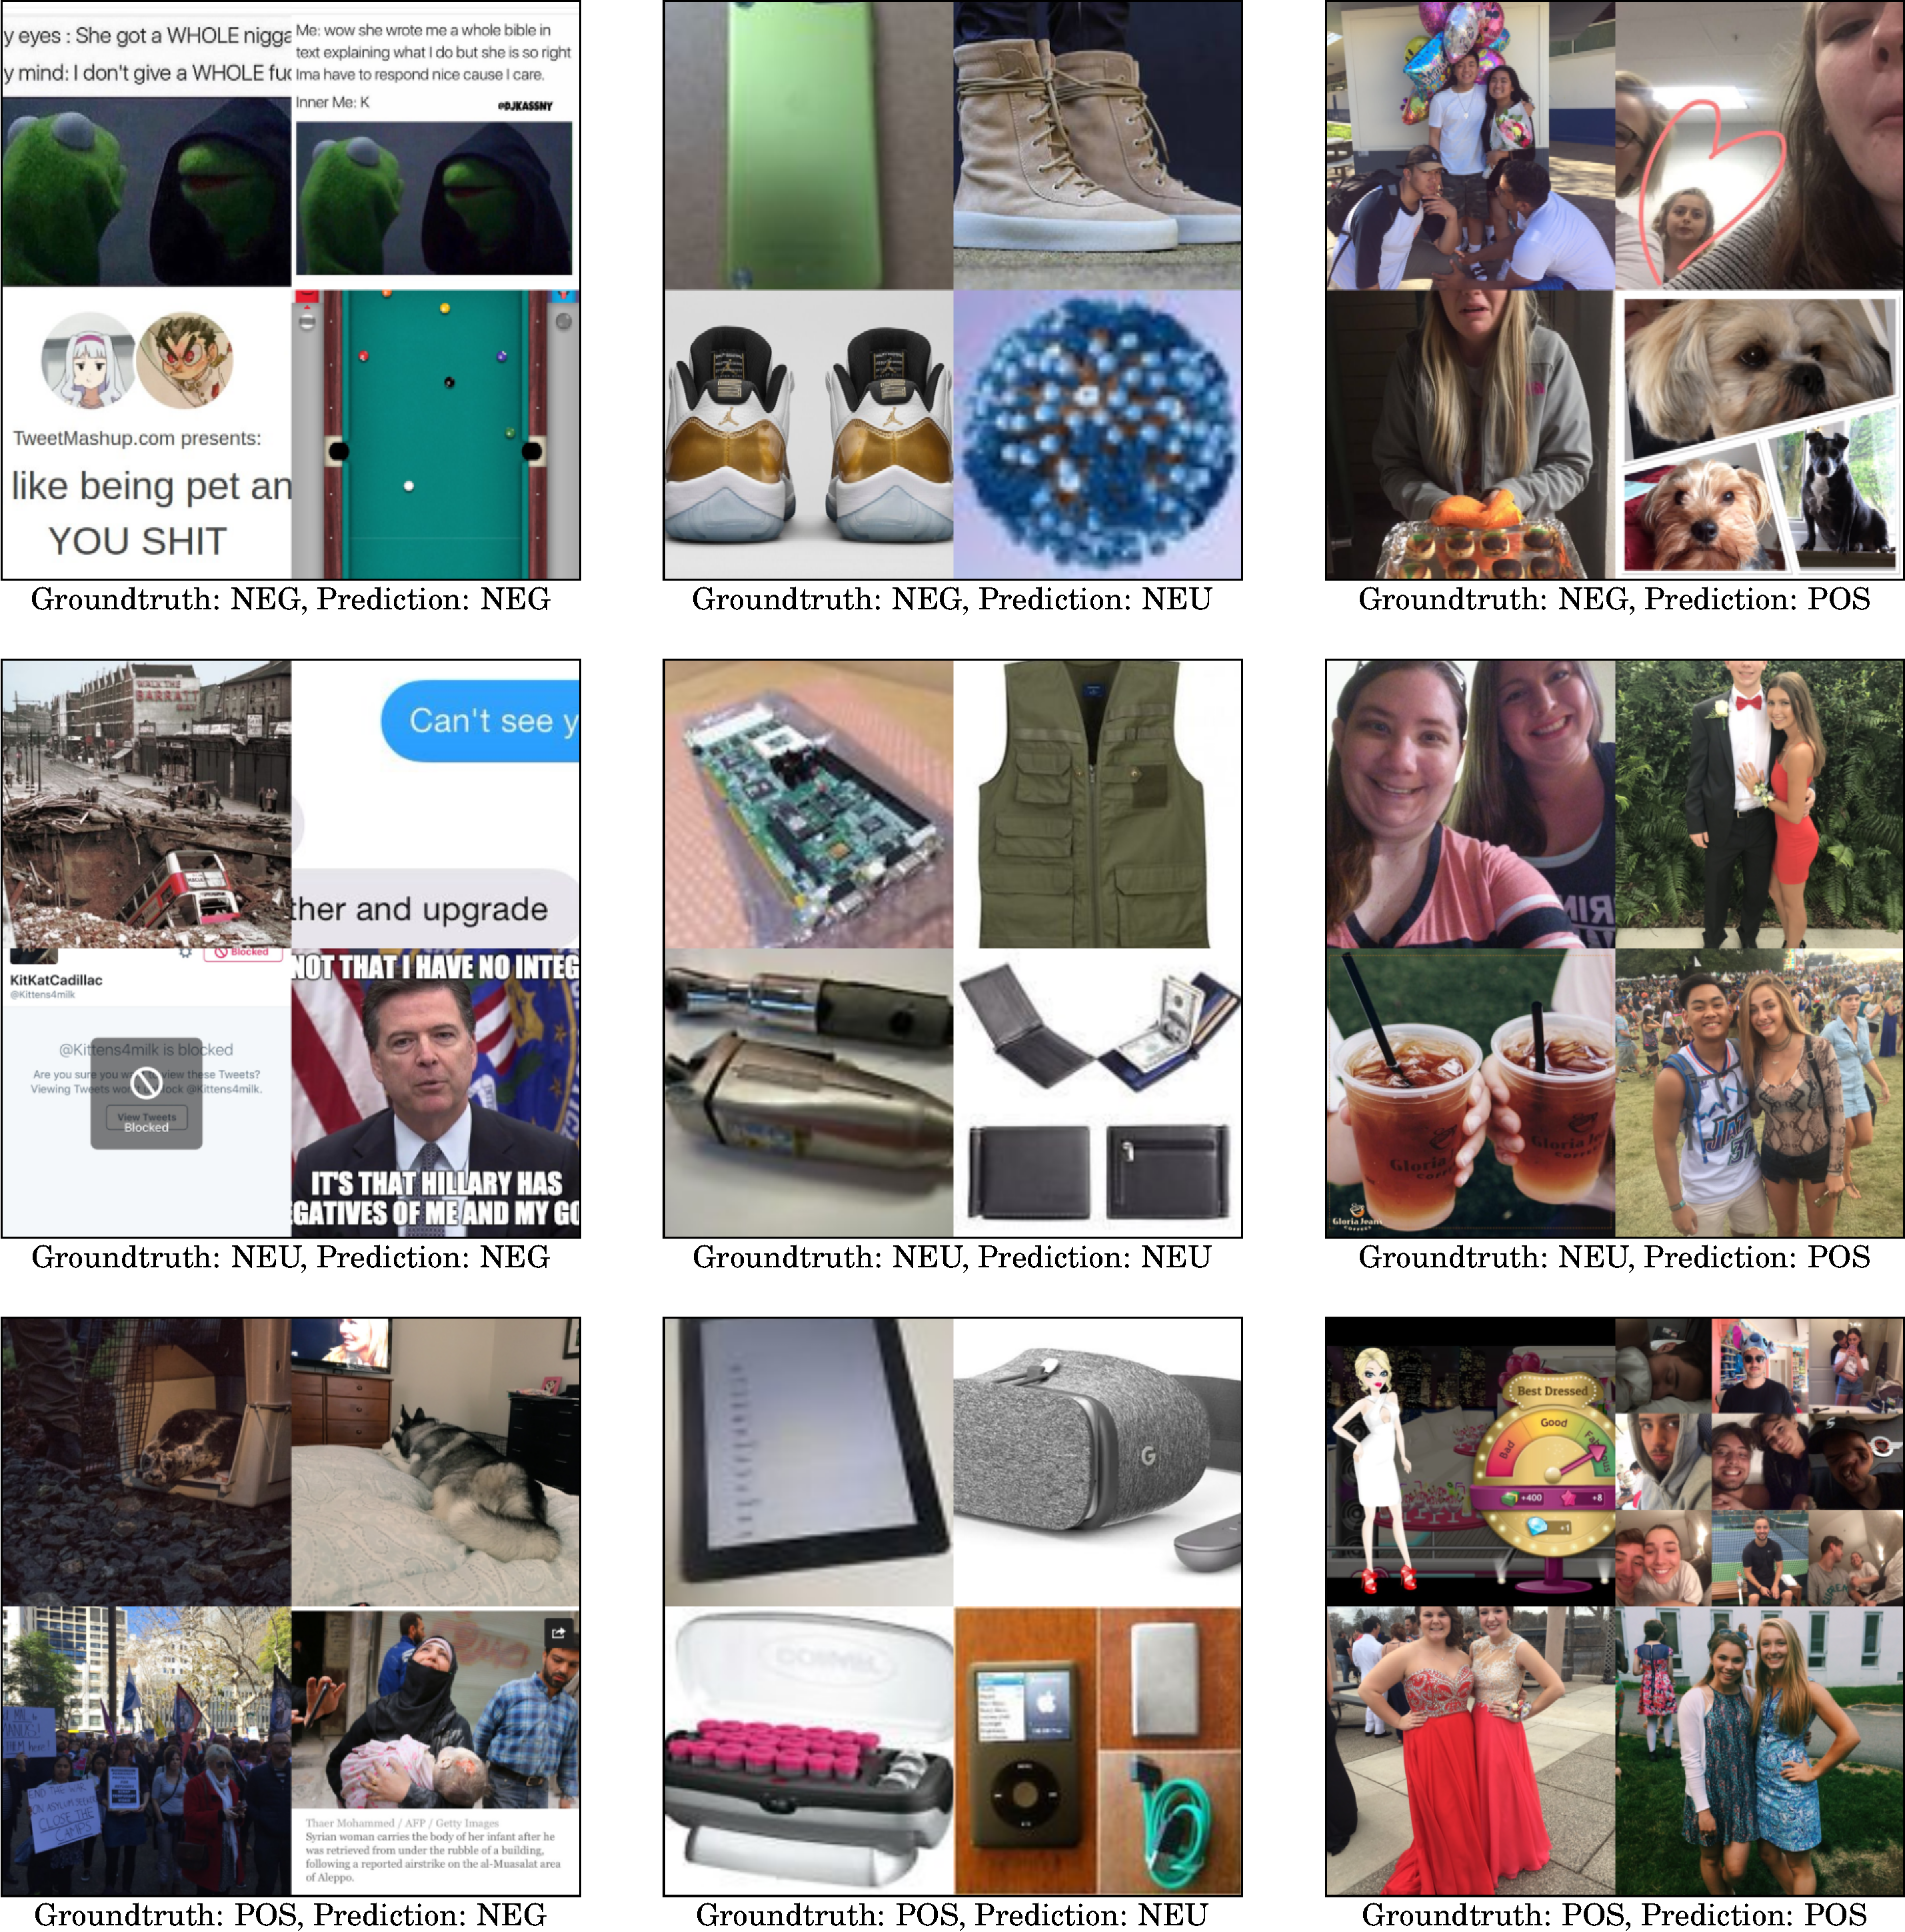
\includegraphics[width=\linewidth]{confusion-images}
\caption{The most confident classifications of our model on our \BTSA\, test set, grouped by all possible (groundtruth, predicted class) couples. Rows (from top to bottom) contains images labeled respectively \emph{negative}, \emph{neutral} and \emph{positive} on the basis of textual sentiment analysis. Columns (from left to right) contain images visually classified respectively as \emph{negative}, \emph{neutral} and \emph{positive} by our model.
%From a qualitative point of view, notice that in several cases the sentiment polarity of the images is better represented by the prediction of our model than the sentiment polarity inferred from the text associated to the images. Since the textual sentiment analysis was used to label both testing and training images, this, on one hand, explains the low accuracy upper bound obtained by our model on the {\BTSA} test set and, on the other hand, confirms that we used sufficiently large set of training data to allow the deep network to handle noisy labels.
}
\label{fig:vsa:confusion-images}
\end{figure}

Many papers on visual sentiment analysis report the 5-fold cross-validation accuracy on the Twitter Testing Dataset~\cite{campos2017pixels,islam2016visual,li2018image,you2015robust}, in which the prediction of each fold is computed with a model fine-tuned on the other four folds. In order to compare to those approaches, we also tested our models in this setting, and we reported the 5-fold accuracy obtained in Table \ref{tab:Twitter882_5fold}.
However, we think that this measure is inappropriate for our cross-media approach since it tends to highlight how well a pretrained model adapts to a specific task or dataset. In fact, as evidenced by the results, models trained on generic (not sentiment-related) datasets, like AlexNet and VGG-19, not necessarily perform worse than the same models previously finetuned on a sentiment-related dataset.
% Possiamo vedere dalla Tabella bla un finetuning intermedio su dati sentimentali non necessariamente produce dei miglioramenti nella 5-fold accuracy.
For example our best approach ({\ourFtVGG} FT-A), achieves a 5-fold accuracy of $0.896$ on the five agree subset, that corresponds only to an improvement of $1.5\%$ with respect to VGG-19 trained on a generic dataset.
Moreover, our technique is based on a cross-media approach, i.e. it relies on labels not coming from a visual inspection of the images. Thus, we think that a fine-tuning of our models on manually labeled images is inappropriate for our goal.
In any case, also in this test setting, our models outperform other state-of-the-art visual classifiers, such as PCNN, DeepSentiBank and MVSO, which were trained on high-quality sentiment-related dataset.

Taken together, these results indicate that our cross-media learning approach is a first, important step towards building systems able to learn the sentiment polarity of images autonomously from the Web.

%Differently by other visual sentiment classifiers

% In order to compare the performance of our model to other state-of-the-art methods, we also performed a 5-fold cross-validation on the testing subsets (as also done in \cite{Campos2016,islam2016visual,li2018image,you2015robust}), in which we compute the prediction of each fold with a model fine-tuned again on the other four folds. Results for 5-fold cross-validation are reported in Table \ref{tab:Twitter882_5fold}.
\begin{table}
\small
\newcolumntype{R}{>{\raggedleft\arraybackslash}X}
\begin{tabularx}{\linewidth}{llRRR}
\toprule
                &                           & \multicolumn{3}{c}{\textsc{Twitter Testing Dataset}} \\
                                              \cmidrule(lr){3-5}
\textsc{Method} & \textsc{Training Datasets} & \textsc{5 agree} & \textsc{$\geq 4$ agree} & \textsc{$\geq 3$ agree} \\
\midrule
\multicolumn{5}{l}{\textbf{Approaches without intermediate fine-tuning}} \\
\midrule
GCH~\cite{siersdorfer2010analyzing}              {\footnotesize (from~\cite{you2015robust})} \tnote{$\ast$}  &   -   &   0.684   &   0.665   &   0.66    \\
SentiBank~\cite{borth2013large}  {\footnotesize (from~\cite{you2015robust})} \tnote{$\circ$} &   -   &   0.709   &   0.675   &   0.662   \\
LCH~\cite{siersdorfer2010analyzing}              {\footnotesize (from~\cite{you2015robust})} \tnote{$\ast$}  &   -   &   0.710   &   0.671   &   0.664   \\
GCH+ BoW~\cite{siersdorfer2010analyzing}         {\footnotesize (from~\cite{you2015robust})} \tnote{$\ast$}  &   -   &   0.710   &   0.685   &   0.665   \\
LCH+ BoW ~\cite{siersdorfer2010analyzing}        {\footnotesize (from~\cite{you2015robust})} \tnote{$\ast$}  &   -   &   0.717   &   0.697   &   0.664   \\
Sentribute~\cite{yuan2013sentribute}   {\footnotesize (from~\cite{you2015robust})} \tnote{$\circ$} &   -   &   0.738   &   0.709   &   0.696   \\

CNN~\cite{you2015robust} \tnote{$\bullet$}   &   Flickr (VSO)    &   0.783   &   0.755   &   0.715   \\
AlexNet {\footnotesize (from~\cite{campos2017pixels})} \tnote{$\bullet$}   &  \gls{ilsvrc}12   &   0.817   &   0.782   &   0.739   \\
PlaceCNN~\cite{zhou2014learning}                {\footnotesize (from~\cite{campos2017pixels})} \tnote{$\bullet$}   &   Places205    &   0.830   &   -   &   -   \\
GoogleNet~\cite{szegedy2015going}   {\footnotesize (from~\cite{islam2016visual})}  \tnote{$\bullet$}   &   \gls{ilsvrc}12   &   0.861   &   0.807   &   0.787   \\
HybridNet \tnote{$\bullet$}   &   \gls{ilsvrc}12 + Places205   &   0.867   &   0.814   &   0.781   \\
VGG-19 \tnote{$\bullet$}   &   \gls{ilsvrc}12  &   0.881   &   0.835   &   0.800   \\

\midrule
\multicolumn{5}{l}{\textbf{Approaches using an intermediate fine-tuning}} \\
\midrule

PCNN~\cite{you2015robust} \tnote{$\bullet$}   &   Flickr (VSO) + \emph{ft} Flickr (VSO)  &   0.773   &   0.759   &   0.723   \\
DeepSentiBank~\cite{chen2014deepsentibank} {\footnotesize (from~\cite{campos2017pixels})} \tnote{$\circ$}\, \tnote{$\bullet$} &   \gls{ilsvrc}12 + \emph{ft} Flickr (VSO)  &   0.804   &   -   &   -   \\
MVSO [EN]~\cite{jou2015visual}   {\footnotesize (from~\cite{campos2017pixels})} \tnote{$\circ$}\, \tnote{$\bullet$} & DeepSentiBank~\cite{chen2014deepsentibank} + \emph{ft} MVSO-EN \cite{jou2015visual}  &   0.839   &   -   &   -   \\
\ourFtAlex\, FT-A (Ours) \tnote{$\bullet$}   &   (\gls{ilsvrc}12 + Places205) + \emph{ft} \BTSA    &   0.864   &   0.830   &   0.800   \\
\ourFtAlex\, FT-F (Ours) \tnote{$\bullet$}   &   (\gls{ilsvrc}12 + Places205) + \emph{ft} \BTSA   &   0.873   &   0.832   &   0.810   \\
\ourFtVGG\, FT-F (Ours) \tnote{$\bullet$}   &   (\gls{ilsvrc}12 + Places205) + \emph{ft} \BTSA   &   0.889   &   0.857   &   0.815   \\
\ourFtVGG\, FT-A (Ours) \tnote{$\bullet$}   &   (\gls{ilsvrc}12 + Places205) + \emph{ft} \BTSA &   \textbf{0.896   }&  \textbf{0.866}  &   \textbf{0.820}  \\

\midrule
\end{tabularx}
$\ast=$ based on low-level features, $\circ=$ based on mid-level features, $\bullet=$ based on deep learning
\footnotesize
%\item[$\ast$]  Approch based on low-level features
%\item[$\circ$]  Approch based on mid-level features
%\item[$\bullet$] Approch based on deep learning

\caption{5-Fold Cross-Validation Accuracy of different methods on Twitter Testing Dataset. \emph{tr} stands for `trained'; \emph{ft} stands for `fine-tuned'. Note that in these experiments \emph{all} the deep models are again fine-tuned on four folds of the Twitter Testing Dataset. During cross-validation we fine-tuned all the weights of our FT models.}
\label{tab:Twitter882_5fold}
\end{table}

% \subsubsection{Results on Phototweet Sentiment Benchmark(?)} %LUCIA%rivedere il titolo e decidere se inserire gli exp
% \cite{borth2013large}
% Ground-truth obtained by AMT annotation

%-------------------------------------------------------------------------
\section{Conclusions}
\label{sec:vsa:conclusion}

%The aim of this work is to explore the possibility of
This application paper deals with the problem of
training a visual sentiment classifier from a large set of multimedia data, without the need of human annotators.
We leveraged on a cross-media learning approach showing that even if the textual information associated to Web images is often noisy and ambiguous, it is still useful for learning robust visual classifiers. % (assuming to have  collections of data large enough to balance the noise in the training labels).
To this scope, we collected and used more than 3 million tweets, and we experimentally shown that our approach is effective for learning visual sentiment classifier in the wild.
We publicly released all the collected data and our trained models for future research and applications.%, as incentive
%Future work will investigating \emph{emotion} visual analysis

%  Web images are often associated with  textual descriptions. Even though such textual information is not .. it is still useful for learning robust classifiers.

% use the massive amount of user-generated data available on the Web in place of human-labeled data. %we contribute to this research thread with a study